\subsection{Frontend Design}\label{design-frontend}
Bei der Architektur und dem Design unterscheiden wir zwischen Backend
(Web Services) und dem Frontend (Android App). Beide Systeme werden parallel und
unabhängig mittels Swagger API Spezifikation entwickelt (siehe \fullref{service-api}).
Durch diesen Swagger Contract als klare Barriere lassen sich Entscheide betreffend
Architektur und Design separat treffen.
Zuerst behandeln wir das Frontend, danach das Backend.
\subsubsection{Design-Klassendiagramm}\label{design-klassendiagram}
\begin{figure}
  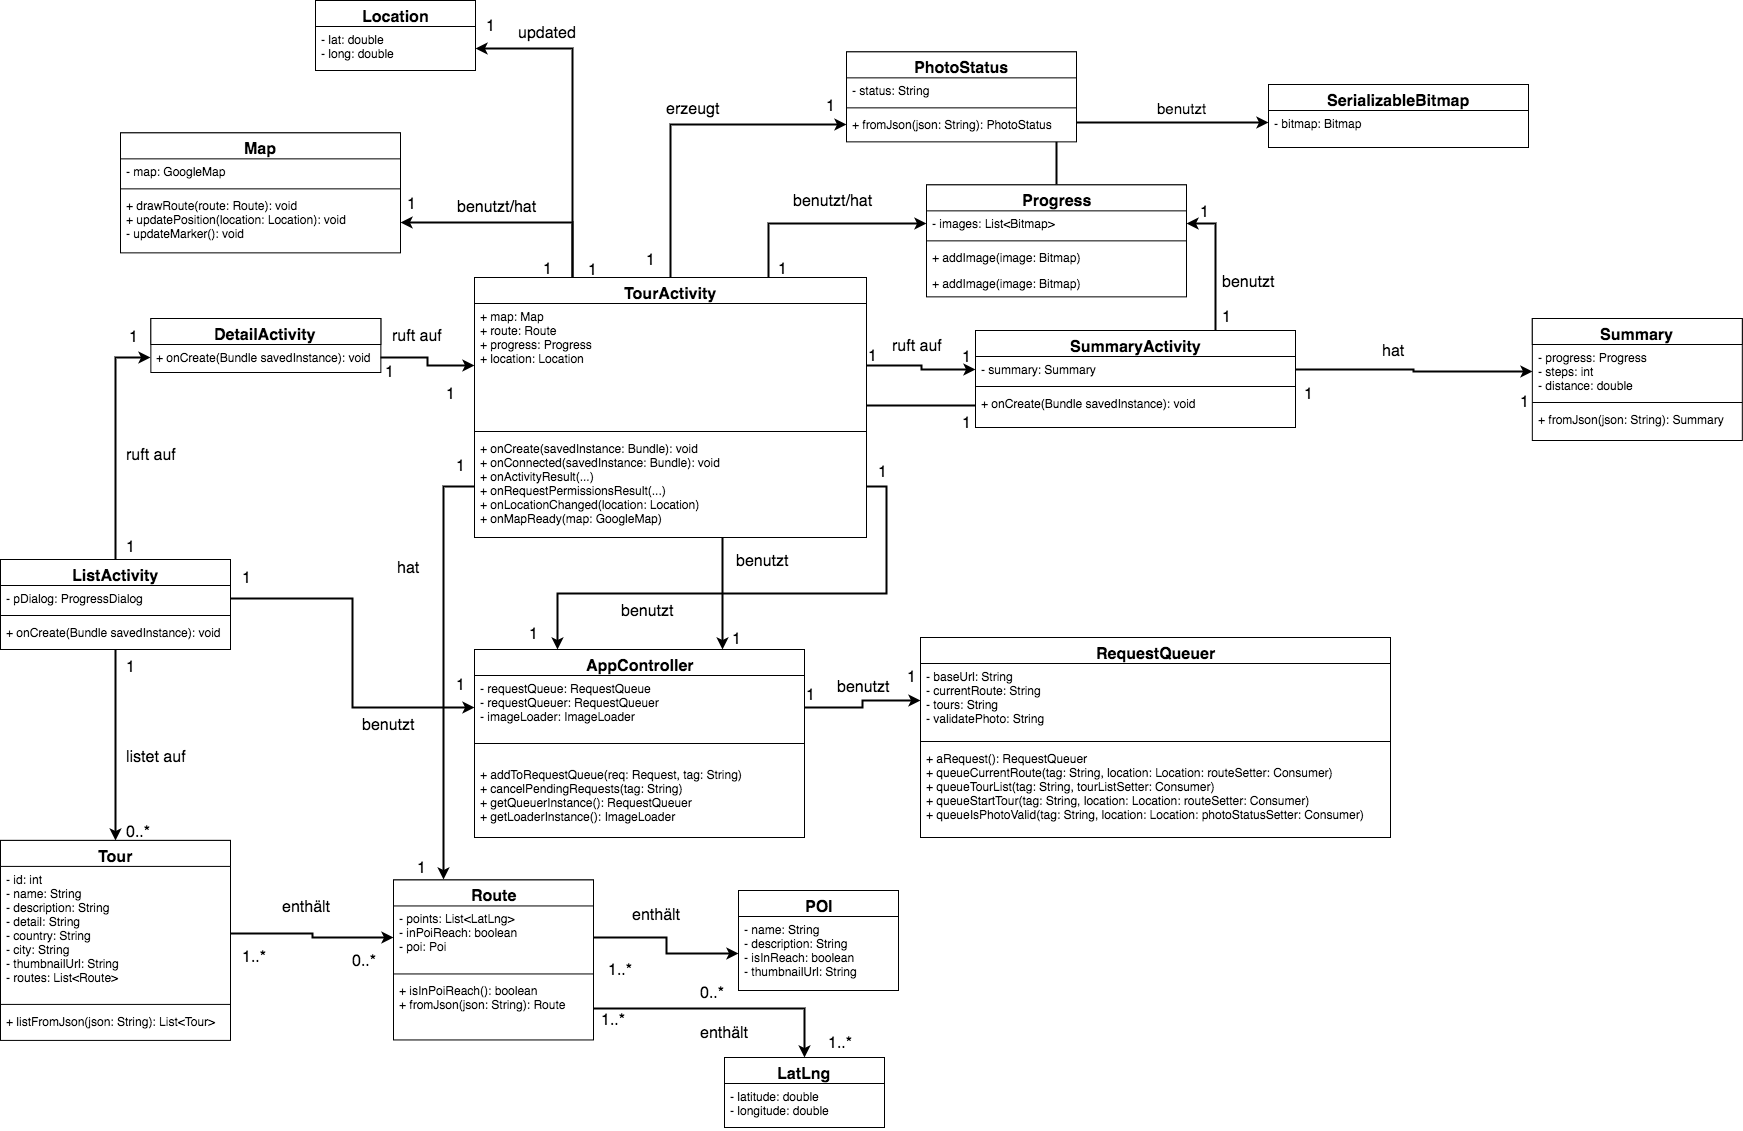
\includegraphics{classdiagram_frontend}
  \caption{Klassendiagramm der App}
\end{figure}

\newpage
\subsubsection{Klassenverantwortlichkeiten}\label{klassenverantwortlichkeiten}
In der folgenden Tabelle werden die Klassen mit ihren Hauptverantworlichkeiten
gelistet.

\begin{longtabu} to \textwidth { | l | X[l] |  }
\hline
\textbf{Klasse} & \textbf{Verwantwortlichkeit}\\\hline
\endhead
\textbf{AppController} & Der AppController liefert Instanzen von Singletons.\\\hline
\textbf{RequestQueuer} & Der RequestQueuer wird benutzt, um per HTTP mit dem
Server zu kommunizieren.\\\hline
\textbf{ListActivity} & Die ListActivity zeigt eine Liste von Touren an und
reagiert auf Klick-Events.\\\hline
\textbf{DetailActivity} & Die DetailActivity zeigt eine detaillierte Beschreibung
und ein Thumbnail einer Tour.\\\hline
\textbf{TourActivity} & Die TourActivity speichert die aktuelle Route, aktualisiert
die Position des Nutzers, aktualisiert die Karte und löst HTTP Requests aus.\\\hline
\textbf{SummeryActivity} & Die SummaryActivity erstellt eine \textbf{Summary}
und zeigt diese an.\\\hline
\textbf{Tour} & Die Tour kennt all ihre Routen und dient als Datenklasse. \\\hline
\textbf{Route} & Die Route kennt all ihre Koordinaten und dient als
Datenklasse. \\\hline
\textbf{POI} & Die POI ist eine reine Datenklasse und bildet ein POI ab.\\\hline
\textbf{LatLng} & LatLng ist ein Datentyp, welche eine Position auf dem
Erdball abbildet.\\\hline
\textbf{Map} & Die Map dient als Behählter der Google Map und wird benutzt, um
die Karte zu aktualisieren.\\\hline
\textbf{Location} & Location ist eine Repräsentation eines Ortes und kommt aus
Android SDK.\\\hline
\textbf{PhotoStatus} & PhotoStatus ist eine Datenklasse und repräsentiert das
Ergebnis einer Validierung eines Fotos durch das Backend.\\\hline
\textbf{Progress} & Progress dient als Behälter der während einer Tour geschossenen
Fotos.\\\hline
\textbf{Summary} & Summary wird am Ende einer Tour aus Progress generiert und
bietet dem Nutzer eine Zusammenfassung der Tour.\\\hline
\textbf{SerializableBitmap} & SerializableBitmap ist eine Wrapper-Klasse um ein Bitmap. Activities
kommunizieren untereinander mit Intents, welche einen serialisierbaren Anhang haben können.
Dadurch lassen sich Fotos zwischen Activities herumreichen.\\\hline

\end{longtabu}

\newpage
\subsubsubsection{Knowing and Doing}\label{knowinganddoing-frontend}
Im Folgenden betrachten wie die Knowing- und Doing-Verantwortlichkeiten der Klassen.
\begin{longtabu} to \textwidth { | l | X[2, l] | X[8, l] |  }
\hline
\textbf{Klasse} & \textbf{Knowing} & \textbf{Doing} \\\hline
\endhead
\textbf{AppController} & RequestQueuer & Stellt anderen Objekten den RequestQueuer
als Singleton zur Verfügung.\\\hline
\textbf{RequestQueuer} & keine Abhängigkeiten & Wird in den Activities für asynchrone
HTTP Kommunikation benutzt. Der RequestQueuer baut auch die URLs zusammen und bietet
eine API an, um mit Lambdas Callbacks zu setzen. Dieser ruft die mitgereichten
Consumer mit dem Server Response auf, ohne den Aufrufer zu kennen. Dadurch erreichen
wir lose Kopplung und hohe Wiederverwendbarkeit. \\\hline
\textbf{ListActivity} & AppController, Tour & Die ListActivity gibt über den AppController
einen Callback an den RequestQueuer. Dieser Callback füllt eine Liste von Touren,
welche dem User angezeigt wird. Ein Klick auf eine Tour ruft die DetailActivity auf.
\\\hline
\textbf{DetailActivity} & Tour & Die DetailActivity ist eine einfache Ansicht auf
ein Tour-Objekt und zeigt Details einer Tour an.\\\hline
\textbf{TourActivity} & Map, Route, Progress, Location, AppController & Die TourActivity bildet
unseren Haupt-Use-Case ab: Navigation per Karte durch eine Tour. Die TourActivity
registriert sich selber als Callback beim Google Maps Service und beim Google
Play Location Service. Weiterhin wird das Backend regelmässig nach der aktuellen
Route gefragt. Falls sich der User in der Nähe eines POIs befindet, wird die
Kamera App des Smartphones aktiviert.\\\hline
\textbf{SummeryActivity} & Summary, Progress, RequestQueuer & Die SummaryActivity
bekommt von der TourActivity ein Progress-Objekt. Nach einer Anfrage an das
Backend wird eine \textbf{Summary} Activity erstellt und angezeigt.\\\hline
\textbf{Tour} & Route & Die Tour kennt nur ihre Routen und dient als Datenklasse.
Sie kann sich selber aus JSON instanziieren.\\\hline
\textbf{Route} & LatLng & Die Route kennt all ihre Koordinaten und dient als
Datenklasse. Sie kann sich selber aus JSON instanziieren.\\\hline
\textbf{POI} & keine Abhängigkeiten & Die POI ist eine reine Datenklasse und bildet ein POI ab. Sie
kann sich selber aus JSON instanziieren.\\\hline
\textbf{LatLng} & keine Abhängigkeiten & LatLng ist ein Datentyp, welche eine Position auf dem
Erdball abbildet.\\\hline
\textbf{Map} & GoogleMap & Die Map dient als Behälter der Google Map und wird benutzt, um
die Karte zu aktualisieren. Sie kann den Positionsmarker und die Route zum nächsten
POI zeichnen.\\\hline
\textbf{Location} & keine Abhängigkeiten & kein Verhalten \\\hline
\textbf{PhotoStatus} & keine Abhängigkeiten & kein Verhalten \\\hline
\textbf{Progress} & keine Abhängigkeiten & kein Verhalten \\\hline
\textbf{Summary} & Progress & Summary kann sich selber aus \textbf{Progress}
generieren.\\\hline
\textbf{SerializableBitmap} & keine Abhängigkeitren & kann ein Bitmap serialisieren \\\hline

\end{longtabu}

Obwohl \textbf{Activities} andere \textbf{Activites} starten können, müssen sie
lediglich deren Klasse kennen. Durch das Messaging System von Android müssen die
Activities keine Instanzen von anderen Activities halten oder diese selber
erzeugen. Im Klassendiagramm (Abbildung 2) sind die Activities zwar miteinander
verbunden, aber durch das Message System (Intents) sind diese lose gekoppelt.


\subsubsection{Android App Architektur}\label{androidapparchitektur}

Die Architekur der App implementiert eine einfache Version von \textbf{The Clean Architecture} \cite{TCA}.
Im nachfolgenden Abschnitt werden einige wichtige Punkte von \textbf{The Clean Architecture}
erläutert, um die Implementation in TravelBuddy aufzuzeigen. Eine umfassende
Einleitung findet man bei Robert Martin (Uncle Bob) \cite{CC}.
\begin{figure}
  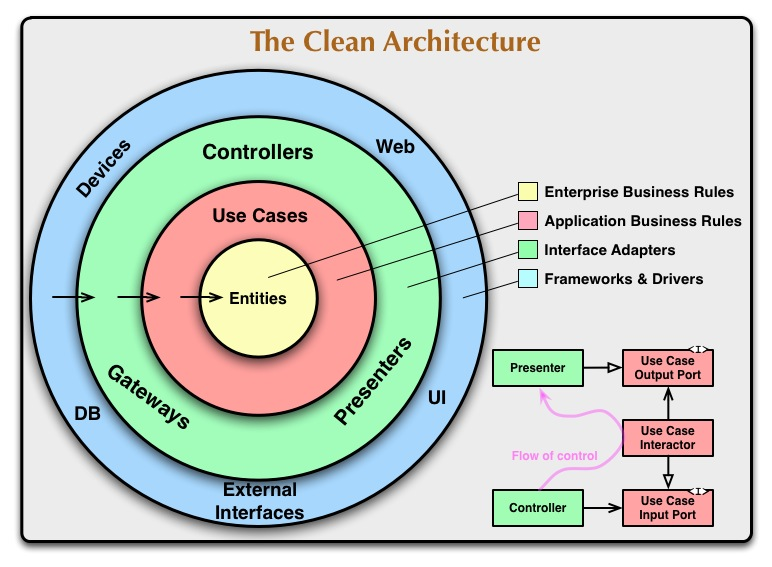
\includegraphics{cleanarchitecture}
  \caption{Schema von The Clean Architecture}
\end{figure}

\subsubsubsection{Abhängigkeiten - Dependency Rule}\label{dependencyrule}
Diese einfache Regel stellt lose Kopplung und gute Testbarkeit sicher.
Die \textbf{Dependency Rule} besagt, dass die Source Code Abhängigkeit nach innen zeigt.
Das heisst, dass eine bestimmte Schicht niemals die äussere Schicht kennt.
Man hat beispielsweise einen HTTP Client (Web) in der äussersten Schicht und
einen Parser (Gateway) in der direkt darunterliegenden Schicht. Nach der
\textbf{Dependency Rule} darf es keine Referenzen im Parser zum HTTP-Client geben.

\subsubsubsection{Bedeutung der Schichten}\label{layers}
\begin{longtabu} to \textwidth { | l | X[l] |  }
\hline
\textbf{Bezeichnung der Schicht} & \textbf{Bedeutung und Beispiele}\\\hline
\endhead
\textbf{Frameworks and Drivers} & Die äusserste Schicht \textbf{Frameworks and Drivers}
ist für die Kommunikation mit der äusseren Welt zuständig. Dazu zählen zum
Beispiel Kommunikation mit dem User per UI, Persistierung von Daten in Datenbanken
oder Kommunikation mit externen Services per HTTP. Die äusserste Schicht beinhaltet
aber auch Frameworks.\\\hline
\textbf{Interface Adapters} & Die nachfolgende Schicht heisst \textbf{Interface Adapters}.
Diese Schicht hat zur Aufgabe, die Daten in eine für die Use-Cases- und Entities-Schicht
möglichst angenehme Form zu bringen.\\\hline
\textbf{Use Case} & Die zweitinnerste Schicht nennt man \textbf{Use Case} Layer.
Hier werden die applikationsspezifischen Businessregeln, also die Use Cases abgebildet.
Die eigentliche Businesslogik existiert also in dieser Schicht. Zu beachten ist aber,
dass es hier nur um Verhalten und nicht um Daten geht.\\\hline
\textbf{Entities} & Die eigentlichen Businessobjekte gehören in die innerste
Schicht, genannt \textbf{Entities}. Diese Schicht hat keine Abhängigkeiten zu
anderen Schichten und beinhaltet die generellen Regeln der Domäne. Bei Änderungen
in äusseren Schichten sind mit hoher Wahrscheinlichkeit keine Änderungen in dieser
Schicht notwendig. Zur Abgrenzung zur oberen Schicht \textbf{Use Case}: Die Schicht \textbf{Entities}
muss nicht angepasst werden, falls sich Use Cases ändern. Dies ist der Fall, da
sich die allgemeinen Domänenregeln in der Regel nicht ändern.\\\hline
\end{longtabu}

\newpage
\subsubsubsection{The Clean Architecture bei TravelBuddy}
Die TravelBuddy App ist ein Spezialfall einer Android App. Da das Team das grösste
Risiko bei der Android-Entwicklung sah, wurde entschlossen, in der App selber so
wenig Businesslogik wie möglich auszuführen.
Dies hat natürlich einen Einfluss auf die Architektur, wie im folgenden Abschnitt aufgezeigt wird.

\begin{longtabu} to \textwidth { | l | X[l] |  }
\hline
\textbf{Schicht} &  \textbf{Zuständigkeiten und Beispiele} \\\hline
\endhead
\textbf{Frameworks and Drivers} & Kümmert sich um Lifecycle der App, die Berechtigungen
und um die Einbettung ins Android Betriebssystem, setzt HTTP Requests ab und reicht
HTTP Responses weiter, aktualisiert Standortdaten, bekommt Bilder von der
Smartphone-Kamera, erhält Karte von der Google Maps App\\\hline
\textbf{Interface Adapters} & Parst Antworten des Servers in String-Form und wandelt
diese Datenobjekte um, transformiert Kartendaten und Standortdaten in für die App
einfach zu handhabbare Form\\\hline
\textbf{Use Case} & Hier kommt der einfache Fall der Android App zugute: Die App
enthält sehr wenig Businesslogik. Die Use Cases sind im Backend implementiert.\\\hline
\textbf{Entities} & Enthält die Datenobjekte, welche die Domänenregeln abbilden:
Eine Tour besteht aus einer Liste von Routen, jede Route hat ein POI zum Ziel\\\hline
\end{longtabu}

\subsubsubsection{Implikationen}\label{implications}
Die Anwendung der \textbf{Clean Architecture} bringt natürlich sowohl Vor- als
auch Nachteile. Die nachfolgende Liste zeigt Implikationen und Auswirkungen der
gewählten Architektur auf das Design und die Umsetzung der App.
\begin{enumerate}
  \item \textbf{Klare Abhängigkeiten:} Durch die klar definierten Abhängikeiten
    lassen sich Kosten und Aufwände von Änderungen/Erweiterungen besser abschätzen:
    Wollen wir beispielsweise die Technologie zur Kommunikation mit dem
    Backend von REST/HTTP auf WebSockets/PubSub ändern, wissen wir, dass sich
    die inneren beiden Schichten nicht ändern. Wir müssen lediglich die äussere
    Schicht anpassen, damit sie WebSockets handhabt. Der Parser, in der direkt
    darunterliegenden Schicht, erhält idealerweise den gleichen Response Body
    und muss nicht angepasst werden.
  \item \textbf{Gute Testbarkeit:} Die Businesslogik ist vollkommen unabhängig
    von verwendeteten Frameworks und der UI. Diese kann ohne eine laufende
    Android Instanz getestet werden. Das führt zu kürzeren Feedback Loops
    bei der Ausführung von Unit Tests und dadurch zur effizienteren Entwicklung
    (ein komplettes Re-deployment entfällt).
    Da in den beiden inneren Schichten keine Abhängigkeit zu externen Systemen
    besteht, lassen sich diese ohne grossen Aufwand (z.B. Testing-Setup) testen.
  \item \textbf{Keine Abhängikeit zum Betriebssytem:} Aus Punkt 1 und 2
    leitet sich dieser Punkt ab: Alle Abhängigkeiten befinden sich um
    äussersten Layer. Falls die App auch auf anderen Systemen lauffähig sein soll, dann muss im Idealfall nur eine Schicht angepasst werden. Durch Projekte wie RoboVM \cite{RV} und Intel Multi OS Engine \cite{MOE} können wir den bestehenden Java Code
    sogar auf iOS Geräten laufen lassen. Unsere App ist damit sogar nur lose
    zum Betriebssystem gekoppelt.
  \item \textbf{Overhead:} Da die App in der ersten Version praktisch keine
    Businesslogik enthalten wird, entfällt die \textbf{Use Case} Schicht.
    Dadurch bleiben eigentlich die anderen drei Layer, die mit der ersten
    Version ebenfalls noch überschaubar ausfallen. Man könnte argumentieren,
    dass diese Architektur etwas zu hoch gegriffen ist für die Anforderungen
    des Prototypen. Im Gegensatz zu Design lässt sich Architektur nicht oder
    sehr schwer inkrementell entwickeln. Wir denken, dass der Aufwand für Änderungen
    der Architektur im späteren Verlauf (etwa durch neue Anforderungen) den
    initialen Mehraufwand rechtfertigt.
\end{enumerate}

Durch die gewählte Architektur erreichen wir gute Testbarkeit mit klaren
Abhängigkeiten. Der Mehraufwand wird dadurch gerechtfertigt, dass Änderungen
von Technologien nur kleine, kalkulierbare Anpassungen zur Folge haben.

\subsubsubsection{Tatsächliche Umsetzung}\label{implementation_frontend}
Die tatsächliche Implementation weicht leicht von der geplanten Architektur ab. Das Team hat den
Aufwand zur vollständigen Entkopplung der äussersten Schicht \textbf{Frameworks and Drivers} abgeschätzt
und schliesst, dass der Mehrwert in diesem Fall den Schritt nicht rechtfertigt.

Um die \textbf{Frameworks and Drivers} Schicht vom Rest der App zu entkoppelt, müssten viele Helper-, Wrapper- und
Facaden-Klassen eingeführt werden. Da die Aufrufe von externen Libraries wie dem HTTP Client Volley
oder der JSON-Parsing Library GSON nur punktuell stattfinden, nehmen wir die Verletzung der \textbf{Dependency Rule}
bewusst in Kauf.
Die vollständige Entkopplung der \textbf{Frameworks and Drivers} Schicht kann, wenn auch mit mehr Aufwand,
zu einem späteren Zeitpunkt durchgeführt werden. Dieser Punkt gehört definitiv zu den Erweiterungsmöglichkeiten
und ist ab einer gewissen Grösse des Projekts obligatorisch.

Die Wahl von guten Abstraktionen und Einhaltung der \textbf{Dependency Rule} ist uns hingegen bei den beiden
inneren Schichten gelungen. Nur durch Betrachten der \textbf{Entitites} werden die Domänenregeln sofort klar,
die Klassen selber haben alle geringe bis keine äusseren Abhängikeiten.
Die \textbf{Use Case} Schicht ist teils in den Activities verwoben. Dies akzeptieren wir bewusst,
da die Businesslogik grösstenteils auf dem Server stattfindet und die Activities auf Input reagieren.
Ausserdem bestehen die Activities fast ausschliesslich aus einer Auflistung von registrierten Callbacks,
was der Lesbarkeit des Codes nicht schadet.

\subsubsubsection{Erwähnenswerte Designentscheide}\label{mentionabble}
Im Folgenden werden noch interessante Designentscheide betrachtet.

Da die Qualität einer mobile App stark von der Benutzerfreundlichkeit abhängt, gibt es einige 
Prinzipien bei der Entwicklung zu beachten. Ein wichtiger Punkt ist der, dass die App 
\textbf{zu jeder Zeit} auf Benutzereingaben reagieren muss. Bei Android wird das mit \textbf{asynchronen}
Operationen realisiert. HTTP Requests beispielsweise werden im Hintergrund ausgeführt, während der User
die teilweise aufgebaute Tourliste betrachtet kann. Die restlichen Tours werden dann einfach nachgeladen.
Diese Asynchronität bringt einige Herausforderungen mit sich:

\begin{itemize}
    \item Die Synchronisation von asynchron ausgeführten Operationen ist aufwendig.
    \item Der Code ist nicht mehr synchron und wird schwieriger zu lesen.
\end{itemize}

\newpage
Diese Probleme haben wir im Frontend mit dem \textbf{RequestQueuer} gelöst. Die Idee ist, dass der 
RequestQueuer eine simple API zur Erstellung von HTTP Requests anbietet. Dabei kann der Client 
(Benutzer des RequestQueuers) zwei Callbacks übergeben. Die beiden Callbacks werden dabei als
Lambda Expressions übergeben und können mit einem erfolgreichen oder einem erfolglosen Ausgang des HTTP 
Requests umgehen. Ähnliches bieten bereits diverse JavaScript Libraries.

Betrachten wir das Beispiel \textbf{"Frage aktuell kürzeste Route zum nächsten POI ab"}:
\begin{verbatim}
public void queueCurrentRoute(String TAG, 
    Location location, Consumer<RouteResponse> routeSetter) {

    String url = UrlBuilder.anUrl().currentRoute(
        new LatLng(location.getLatitude(),  location.getLongitude())).build();

    StringRequest req = new StringRequest(url,
        response -> routeSetter.accept(RouteResponse.fromJson(response)),
        error -> onError(TAG, error, url));

    AppController.getInstance().addToRequestQueue(req, TAG);
}
\end{verbatim}

Hier wird die aktuelle Route als HTTP Request mit dem \textbf{RequestQueuer} auf die Queue des HTTP Client
Volley gelegt. Android selber entscheidet, wann der HTTP Request ausgeführt wird. Bei einer erfolgreichen
Antwort des Servers wird der Callback \textbf{routeSetter} mit der geparsten Antwort aufgerufen.
Bei einem Fehlschlag wird ein Fehler-Callback \textbf{onError} aufgerufen.

Ein Aufruf dieser Methode sieht dann wie folgt aus:

\begin{verbatim}
RequestQueuer.aRequest().queueCurrentRoute(TAG, location, this::onReceiveCurrentRoute);
\end{verbatim}

Mit einem Callback \textbf{onReceiveCurrentRoute}:

\begin{verbatim}
private void onReceiveCurrentRoute(RouteResponse routeResponse) {
    mMap.drawRoute(routeResponse.getRoute());
}
\end{verbatim}

Dadurch verschwindet die Logik der HTTP Requests aus den Activities, generelles Error-Handling sowie
Code-Reuse werden möglich und der Code wird lesbarer.

Eine Erweiterungsmöglichkeit davon wäre, ein Äquivalent zu Promises zu verwenden. Dabei wird
kein Callback registriert, sondern ein Container zurückgeben. Dieser Container stellt des Resultat 
einer asynchronen Operation dar und kann drei Zustände haben: \textbf{Pending|}, \textbf{Fulfilled} oder
\textbf{Rejected}. Dabei steht die Logik einer asynchronen Operation an der gleichen Stelle im Code,
was die Kohäsion erhöht.

\newpage
\subsubsubsection{Activities}\label{activities}
Die App selber besteht aus drei Haupt-Activities. \textbf{Activities} ist ein
Konzept von Android, sie bilden eine User-Ansicht ab und bilden des Skelett
der App. Abbildung 4 veranschaulicht alle möglichen Zustände und deren
Änderungen.
\begin{figure}
  \centering
  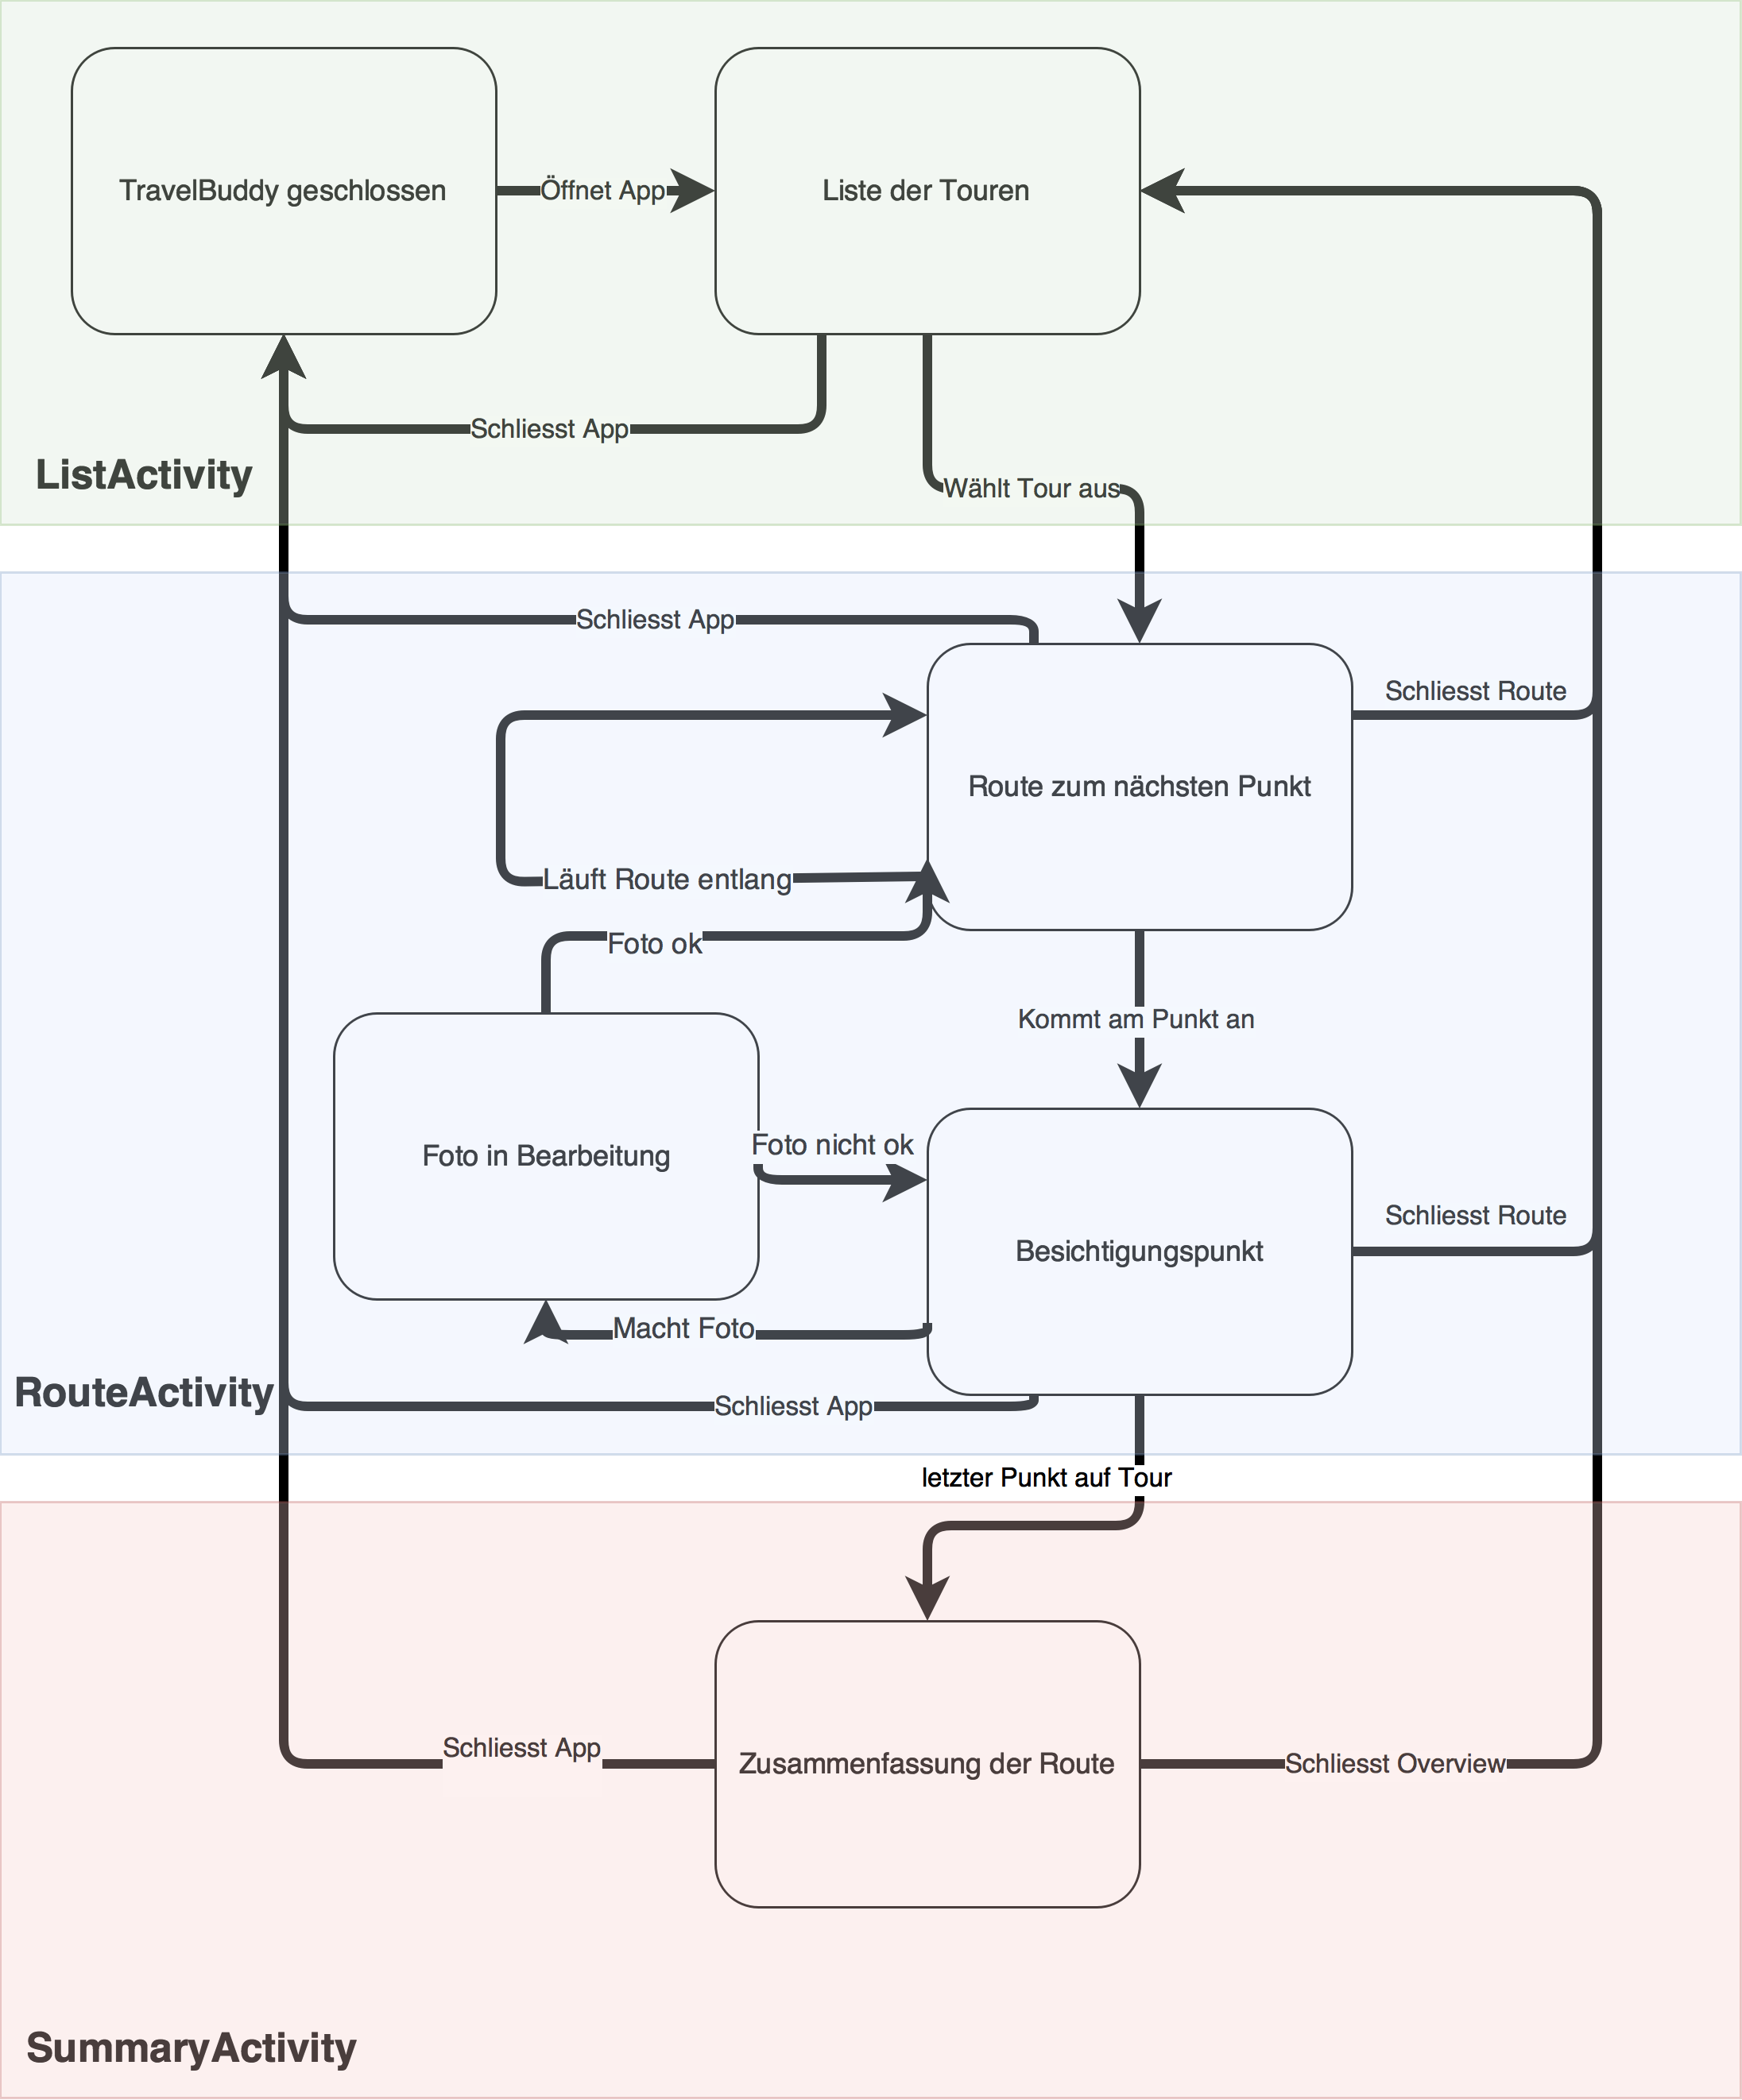
\includegraphics[height=19cm]{state-diagram}
  \caption{Zustandsänderungsdiagramm}
\end{figure}
